\scanpage{179}
\mspage{14}
% archive sheet number: 178
3. \uline{Démonstration de} 1.4 \uline{dans le cas de la dim. relative} 1

\deleted{Soit $W$ l'\unsure{anneau}. On peut} \inserted{\unsure{Soit $W$ un anneau}} de Cohen de corps résiduel $k$, et choisissons un hom $W\to A$ (où $S=\operatorname{Spec}A$) \deleted{\unsure{induisant}} \inserted{\unsure{prolongeant}} l'identité sur $k$.
Nous allons admettre pour l'instant le lemme-clef suivant, qui sera prouvé dans \deleted{\illegible{1}} l'exposé \uline{VII} \deleted{\unsure{en}} à l'aide de la théorie des \inserted{\unsure{modules formels de}} \uline{Schlessinger}.

% A vertical emphasis stroke runs along the lemma in the left margin.
\uline{Lemme} 3.1. Sous les conditions a) b) c) de 1.4, avec $\dim X_s=1$, on peut trouver une algèbre \deleted{locale noethérienne} \inserted{$A_0$ sur $W$}, isomorphe à un anneau de séries formelles
\[
A_0\simeq W[[t_1,\ldots,t_N]],
\]
\deleted{et un} un schéma $\bar X_0$ sur $A_0$, un sous schéma $Y_0$ de $\bar X_0$, et un morphisme $\{f:S=\operatorname{Spec}A\longrightarrow S_0=\operatorname{Spec}A_0\}$ de telle façon que les conditions suivantes soient vérifiées :

(i) $(\bar X_0,Y)$ sur $A_0$ satisfait les conditions a) b) c) de 1.4, i.e. $\bar X_0$ est projectif et plat sur $S_0$, $(\bar X_0)_{\bar s_0}$ -- ($s_0$, le pt fermé de $S_0$) -- est une courbe \deleted{\unsure{de}} algébrique \deleted{\unsure{dim}} n'ayant au pis que des points singuliers ordinaires, $Y$ est \deleted{la réunion} \inserted{un diviseur relatif sur $\bar X_0/S_0$} \deleted{\unsure{de quelques}} \deleted{\unsure{de ses} \unsure{clos|classes} formés de sections $(g_\alpha)_{1\leq\alpha\leq r}$ (éventuellement vide) de $\bar X_0$ sur $S_0$, telles que $g_\alpha(s_0)$ est un pt lisse de $(\bar X_0)_s$ pour tout $\alpha$.}

(ii) Soit $(x_i)_{i\in I}$ la famille des pts \deleted{\unsure{fins|fermés}} singuliers de $X_s$ (ils sont \deleted{rat/$k=k(s)$ par (i)).} \unsure{sép|sep}/$k=k(s)$ par (i); -- cf EGA \uline{V} -- donc rat/$k$). Il existe une famille de diviseurs \inserted{$\unsure{>0|\geq0}$} $(D_i)_{i\in I}$, \deleted{\unsure{réguliers}} sur $S$, telle que \deleted{la famille} $\operatorname{div}(\uline{p})+\sum D_i+$ est à croisements normaux et \deleted{les} \inserted{\unsure{des pts}} $D_i$ de car. génériques nulles [de façon \deleted{\unsure{plus}} précise, on peut supposer \inserted{$I=[1,\unsure{r|n}]$ \unsure{et}} que les $D_i$ sont de la forme $\operatorname{div}(t_i)$], [de telle façon que pour $t\in S_0$, on ait $t\in D_i$ ssi il existe une générisation $x'_i$ de $x_i$ au dessus de $t$, \deleted{avec} \inserted{telle que} $\bar X_0$ \inserted{est} \unsure{non} lisse sur $S_0$ en $x'$.] En particulier, $U_0=S_0-\bigcup\operatorname{Supp}D_i$ est le plus grand ouvert au dessus duquel \deleted{\unsure{$S$}} $\bar X_0$ soit lisse.
\margin{\unsure{p|?}\unsure{!}}
\figure{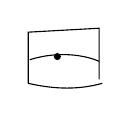
\begin{tikzpicture}[x=1cm,y=1cm]
\draw (0,0) -- (0,0.65) -- (0.9,0.70) -- (0.9,0.05);
\draw (0,0) .. controls (0.35,-0.08) and (0.65,-0.08) .. (0.94,0);
\draw (0.02,0.30) .. controls (0.30,0.39) and (0.64,0.39) .. (0.90,0.28);
\fill (0.37,0.34) circle (0.045);
\end{tikzpicture}}

(iii) Le couple $(\bar X,Y)$ sur $S$ est isomorphe au \deleted{\unsure{couple}} l'image inverse de $(\bar X_0,Y_0)$ sur $S_0$ par $f:S\longrightarrow S_0$.
